\chapter{\label{chapter 4}Evaluation}

In this chapter I will evaluate the convergence time of the iSDX without and with Swift.
I will then examine the vmac partitioning and the number of flow rules required for a fast reroute.

\section{\label{chapter4:Test Setup}Test Setup}

\begin{figure}[h]
\center
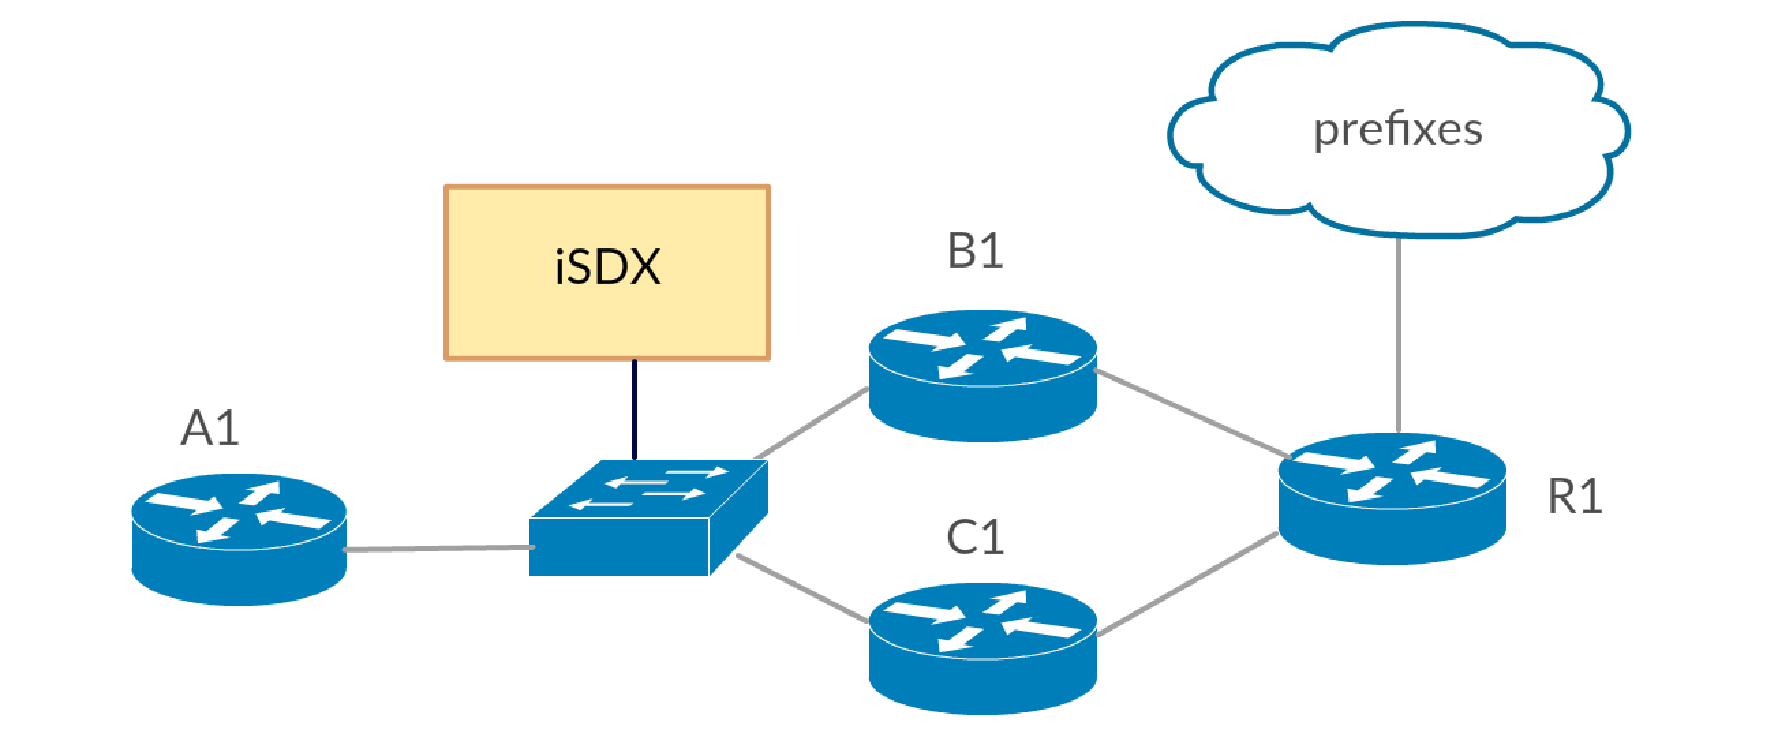
\includegraphics[scale = 0.36]{../Figures/eval_exp_setup.pdf}
\caption{Experiment Setup}
\end{figure}

The test setup has an iSDX with or without Swift connected to three participants. Participants B1 and C1 are connected to the rest of the internet via R1 and advertise up to 500000 prefixes to A1. Participant A1 prefers routes from B1. Remote failure is simulated by setting the link B1 R1 down. If this link is down A1 needs to updates his RIB, check if flow rules have changed and update the virtual next-hop/vmac for every withdrawn prefix.\\ 
The experiment setup is run in mininet. 



\section{\label{chapter4:Convergence time without Swift}Convergence time without Swift}

Convergence time is measured as the time between the first withdraw arriving in the route server and the participant controller finishing to process the last withdraw. To measure the convergence time the built in iSDX log server is used.\\
This convergence time does not take into account the hold timer or the time the participant router takes to process the withdrawals. But since these things are not under the control of the iSDX they are ignored in this evaluation.

\begin{figure}[h]
\center
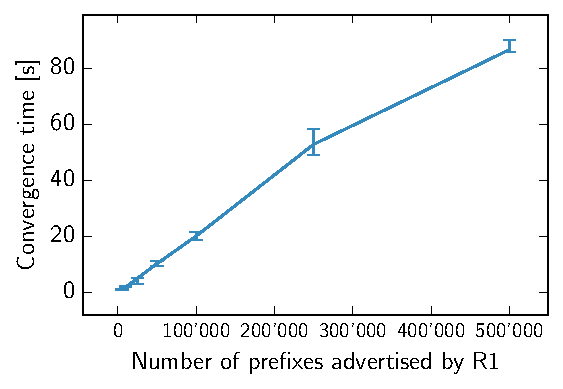
\includegraphics[scale = 1]{../Figures/noswift.pdf}
\caption{Convergence time of the iSDX without Swift}
\end{figure}

\newpage

The convergence time increases linearly with the number of prefixes advertised by R1. \\
At 500'000 prefixes the iSDX takes about 90 seconds to converge. During these 90 seconds A1 sends packet to B1, which then get dropped by B1. 

\section{\label{chapter4:Convergence time with Swift}Convergence time with Swift}

Convergence time is measured as the time between the first withdraw arriving in the route server and the participant controllers FR handler finishing to push the Fast-reroute rules. \\

\begin{figure}[h]
\center
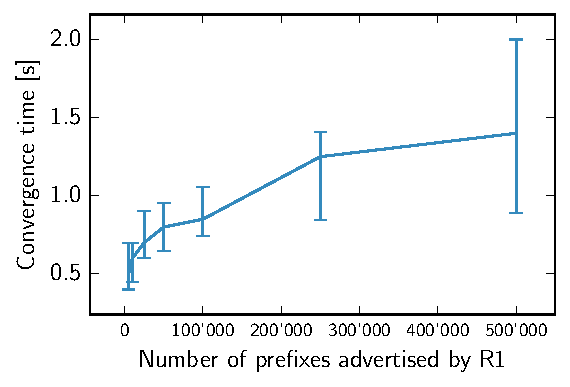
\includegraphics[scale = 1]{../Figures/swift.pdf}
\caption{Convergence time of the iSDX without Swift}
\end{figure}

The convergence time increases slightly with higher number of prefixes. At 500'000 prefixes the iSDX takes about 1.5 seconds to push the FR rules. After these 1.5 seconds packets sent from A1 get redirected to C1 and reach their destination. \\
For 500'000 prefixes the convergence time is reduced by a factor of 60.


\newpage

\section{\label{chapter4:vmac evaluation}vmac evaluation}

Since both the iSDX and Swift use the destination mac address to encode different information, the amount of bits available to  the iSDX and Swift is reduced. In this section the vmac partitioning in its current state will be analyzed.

\begin{figure}[h]
\center
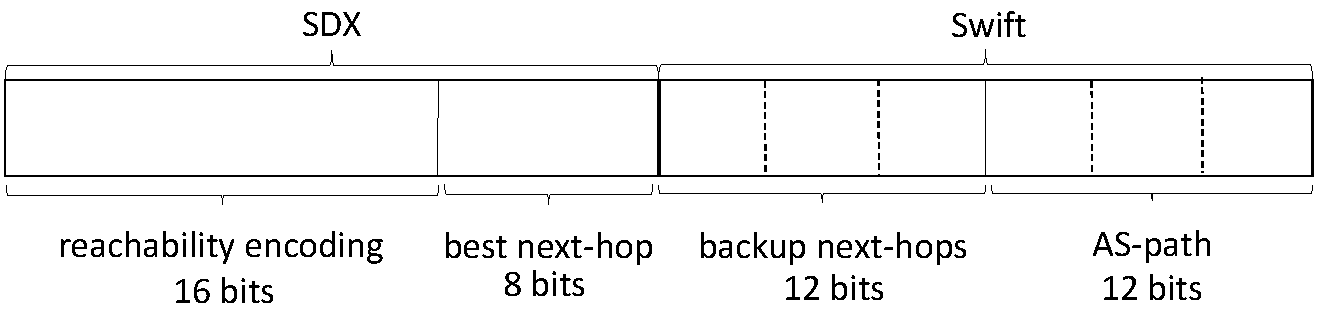
\includegraphics[scale = 0.65]{../Figures/eval_vmac_cropped2.pdf}
\caption{Vmac of the iSDX with Swift}
\end{figure}

In its current state 24 bits are allocated to the iSDX. 16 bits for the reachability encoding and 8 bits for the BGP best next-hop. \\
The amount of bits allocated for the best next-hop limits the number of participants the iSDX with Swift can have. The number of participants is limited to $2^8$ = 256. \\
24 bits are allocated to Swift. 12 bits are used to encode backup next-hops and 12 bits are used for the AS-path encoding. \\
With 12 bits used for the AS-path encoding the encoding has a coverage performance of about 85\%. (see Swift paper Figure 9)\\
12 bits for 3 backup next-hops means 4 bits for each next-hop. This means that every participant can have 16 backup next-hops at most. This is not a lot and after 16 backup next-hops have been assigned some prefixes will end up with no backup next-hop. On the other hand it also limits the number of fast reroute rules. 


\section{\label{chapter4:number of flow rules}number of flow rules}

After a fast reroute message has been received the FR handler pushes reroute rules into the IXP fabric. For every backup next-hop that the participant has stored a rule is pushed. This means the maximum number of rules pushed by a participant after a fast reroute is 16. \\
FR messages get sent to every participant so the maximum number of flow rules for all the participants is 256*16 = 4096. This amount of flow rules is not substantial enough to have a significant impact on the iSDX. With the number of participants limited to 256 and participants having a reasonbale number policies, the flow rule limit for current SDN switches should not be reached. (iSDX paper figure 3 (a) amsix paper figure 9 )\\
